\documentclass{beamer}
\usetheme{Warsaw}

\usepackage{graphicx} % Allows including images
\usepackage{booktabs} % Allows the use of \toprule, \midrule and \bottomrule in tables
\usepackage{listings}
\usepackage[utf8]{inputenc}
\usepackage[overlay,absolute]{textpos}
\usepackage[]{algorithm2e}
\usepackage{amssymb}
\usepackage{tikz}
\usetikzlibrary{arrows, automata}

\AtBeginSection[]
{
\begin{frame}<beamer>
\frametitle{Plan}
\tableofcontents[
  currentsection,
  hideothersubsections
]
\end{frame}
}

\lstset{language=C++,
                basicstyle=\ttfamily,
                keywordstyle=\color{green}\ttfamily,
                stringstyle=\color{red}\ttfamily,
                commentstyle=\color{cyan}\ttfamily,
                morecomment=[l][\color{magenta}]{\#}
}

\setbeamercolor{normal text}{fg=white,bg=black!90}
\setbeamercolor{structure}{fg=white}

\setbeamercolor{alerted text}{fg=red!85!black}

\setbeamercolor{item projected}{use=item,fg=black,bg=item.fg!35}

\setbeamercolor*{palette primary}{use=structure,fg=structure.fg}
\setbeamercolor*{palette secondary}{use=structure,fg=structure.fg!95!black}
\setbeamercolor*{palette tertiary}{use=structure,fg=structure.fg!90!black}
\setbeamercolor*{palette quaternary}{use=structure,fg=structure.fg!95!black,bg=black!80}

\setbeamercolor*{framesubtitle}{fg=white}

\setbeamercolor*{block title}{parent=structure,bg=black!60}
\setbeamercolor*{block body}{fg=black,bg=black!10}
\setbeamercolor*{block title alerted}{parent=alerted text,bg=black!15}
\setbeamercolor*{block title example}{parent=example text,bg=black!15}

\author[Félix-Antoine Ouellet]{Félix-Antoine Ouellet}

\title[Cache\hspace{2em}\insertframenumber/\inserttotalframenumber]{Comportement et exploitation de la cache en multiprogrammation}

\institute{Université de Sherbrooke}

\date{20 novembre 2014}

\begin{document}

\begin{frame}
\titlepage % Print the title page as the first slide
\end{frame}

\begin{frame}
\tableofcontents[hideallsubsections]
\end{frame}

\section{Motivation}
\begin{frame}
\frametitle{Un simple problème}
\framesubtitle{Étape 1}
Générer aléatoirement N entiers et les insérer dans une séquence de sorte qu'ils soient triés en ordre croissant.

Par exemple, 5 1 4 2 donne:
\begin{itemize}
\item[-] 5
\item[-] 1 5
\item[-] 1 4 5
\item[-] 1 2 4 5
\end{itemize}
\end{frame}

\begin{frame}
\frametitle{Un simple problème}
\framesubtitle{Étape 2}
Enlever les éléments de la séquence 1 à 1, et ce, de manière aléatoire.

Par exemple, 1 2 0 0 donne:
\begin{itemize}
\item 1 2 4 5
\item 1 4 5
\item 1 4
\item 4
\end{itemize}
\end{frame}

\begin{frame}
\frametitle{Un simple problème}
\framesubtitle{Résultats}
\begin{center}
\colorbox{white}{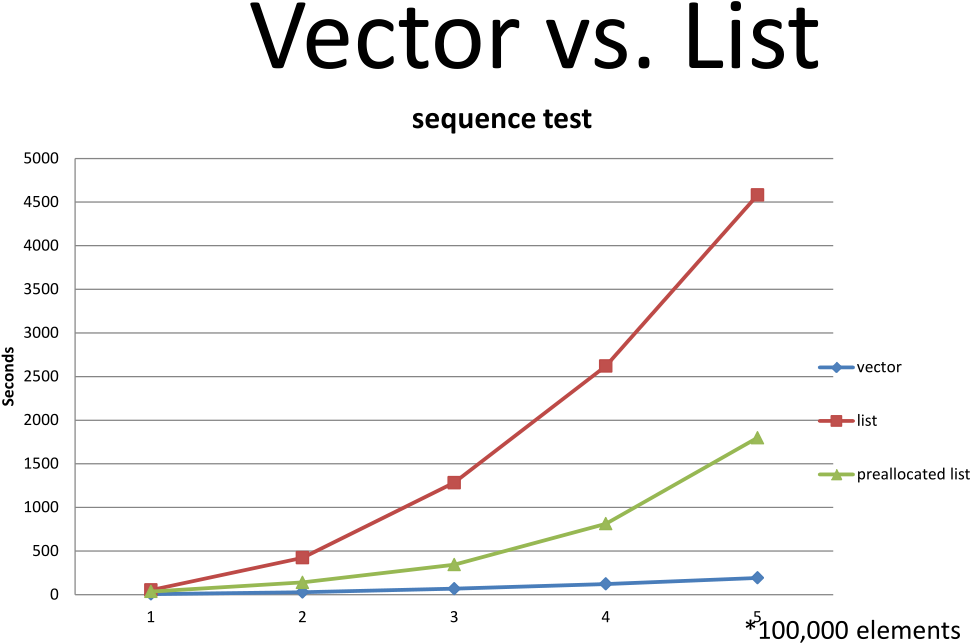
\includegraphics[scale=0.25]{VS.png}}
\end{center}
\end{frame}

\begin{frame}
\frametitle{Modèle académique}
\begin{center}
\begin{tikzpicture}[-,>=stealth',shorten >=1pt,auto,node distance=3cm,
  thick,main node/.style={circle,draw,font=\sffamily\Large\bfseries}]
            
    \draw[white] (0, 0) -- (1, 1) -- (9, 1) -- (10, 0) -- (0, 0);
    
    \draw[white] (4, 5) -- (5, 6) -- (6, 5) -- (4, 5);
    
    \draw[white] (5, 1) -- (5, 5);
\end{tikzpicture}
\end{center}

\begin{textblock}{5}(7, 13.1)
	 Mémoire
\end{textblock}
\begin{textblock}{5}(7.5, 5)
	 CPU
\end{textblock}
\end{frame}

\begin{frame}
\frametitle{Réalité}
\begin{center}
\begin{tikzpicture}[-,>=stealth',shorten >=1pt,auto,node distance=3cm,
  thick,main node/.style={circle,draw,font=\sffamily\Large\bfseries}]
            
    \draw[white] (0, 0) -- (1, 1) -- (9, 1) -- (10, 0) -- (0, 0);
    
    \draw[white] (1, 1.25) -- (2, 2.25) -- (8, 2.25) -- (9, 1.25) -- (1, 1.25);
    
    \draw[white] (2, 2.5) -- (3, 3.5) -- (7, 3.5) -- (8, 2.5) -- (2, 2.5);
    
    \draw[white] (3, 3.75) -- (4, 4.75) -- (6, 4.75) -- (7, 3.75) -- (3, 3.75);
    
    \draw[white] (4, 5) -- (5, 6) -- (6, 5) -- (4, 5);
    
    \draw[white] (5, 1) -- (5, 1.25);
    \draw[white] (5, 2.25) -- (5, 2.5);
    \draw[white] (5, 3.5) -- (5, 3.75);
    \draw[white] (5, 4.75) -- (5, 5);
\end{tikzpicture}
\end{center}

\begin{textblock}{5}(7, 13.1)
	 Mémoire
\end{textblock}
\begin{textblock}{5}(7, 11)
	 Cache L3
\end{textblock}
\begin{textblock}{5}(7, 9)
	 Cache L2
\end{textblock}
\begin{textblock}{5}(7, 7)
	 Cache L1
\end{textblock}
\begin{textblock}{5}(7.5, 5)
	 CPU
\end{textblock}
\end{frame}

\section{Fonctionnement de la cache}
\subsection{Concepts de base}
\begin{frame}
\frametitle{Cache}
\framesubtitle{Illustration}
\begin{columns}
    \begin{column}{0.7\textwidth}
\begin{center}
\begin{tikzpicture}[-,>=stealth',shorten >=1pt,auto,node distance=3cm,
  thick,main node/.style={circle,draw,font=\sffamily\Large\bfseries}]

    \draw[white] (0, 0) rectangle (4, 0.75);
    \draw[white] (0, 0.75) rectangle (4, 1.5);
    \draw[white] (0, 1.5) rectangle (4, 2.25);
    \draw[white] (0, 2.25) rectangle (4, 3);
    \draw[white] (0, 3) rectangle (4, 3.75);
    \draw[white] (0, 3.75) rectangle (4, 4.5);
    
    \draw[white] (-0.1, -0.03) -- (-0.3, -0.03) -- (-0.3, 4.5) -- (-0.1, 4.5) node (1) at (-0.7, 2.4) {$M$};
    
    \draw[white] (0, -0.1) -- (0, -0.3) -- (4, -0.3) -- (4, -0.1) node (1) at (2, -0.6) {$B$};
   
\end{tikzpicture}
\end{center}
    \end{column}
    \begin{column}{0.4\textwidth}
\begin{itemize}
\item Comporte $B$ blocs (\textit{cache lines})
\item Taille $M$
\item Chaque bloc à une taille $B/M$
\end{itemize}
    \end{column}
\end{columns}
\end{frame}

\begin{frame}
\frametitle{Accès à la mémoire}
\begin{itemize}
\item En général, les processeurs ne peuvent accéder directement à la mémoire
\item Les accès mémoire se font au travers d'une hiérarchie de caches
\end{itemize}
\end{frame}

\begin{frame}[fragile]
\frametitle{Lecture}
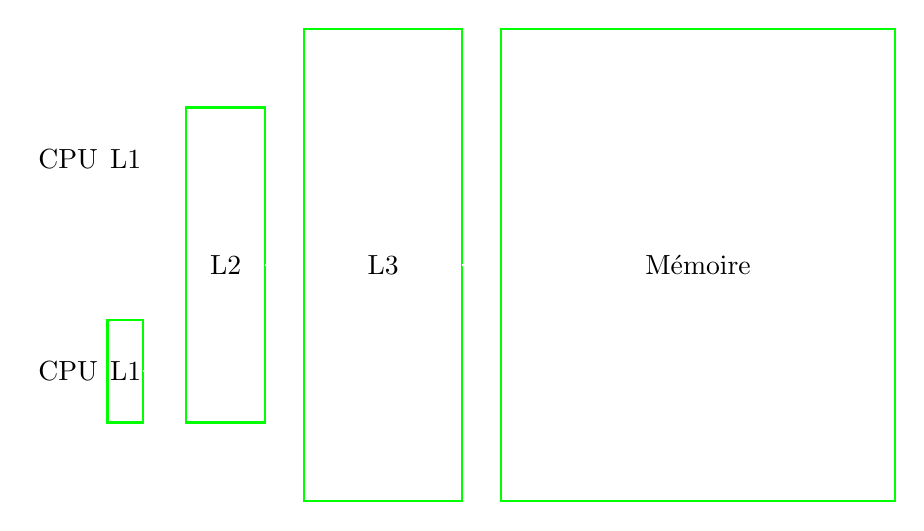
\begin{tikzpicture}[-,>=stealth',shorten >=1pt,auto,node distance=3cm,
  thick,main node/.style={circle,draw,font=\sffamily\Large\bfseries}]

	\draw[white] (0, 0) rectangle (1.45, 1.3);
	\draw[white] (1, 0) rectangle (1.45, 1.3);
	\onslide<2>{\draw[red] (1, 0) rectangle (1.45, 1.3);}
	\onslide<9->{\draw[green] (1, 0) rectangle (1.45, 1.3);}
	\draw[white] (0, 2.7) rectangle (1.45, 4);
	\draw[white] (1, 2.7) rectangle (1.45, 4);
	\draw[white] (2, 0) rectangle (3, 4);
	\onslide<3>{\draw[red] (2, 0) rectangle (3, 4);}
	\onslide<8->{\draw[green] (2, 0) rectangle (3, 4);}
	\draw[white] (3.5, -1) rectangle (5.5, 5);
	\onslide<4>{\draw[red] (3.5, -1) rectangle (5.5, 5);}
	\onslide<7->{\draw[green] (3.5, -1) rectangle (5.5, 5);}
    \draw[white] (6, -1) rectangle (11, 5);
    \onslide<5>{\draw[red] (6, -1) rectangle (11, 5);}
    \onslide<6->{\draw[green] (6, -1) rectangle (11, 5);}
    
    \node (1) at (0.5, 0.65) {CPU};
    \node (2) at (0.5, 3.35) {CPU};
    \node (3) at (1.23, 0.65) {L1};
    \node (4) at (1.23, 3.35) {L1};
    \node (5) at (2.5, 2) {L2};
    \node (6) at (4.5, 2) {L3};
    \node (7) at (8.5, 2) {Mémoire};
    
    \draw[white] (1.45, 0.65) -- (2, 0.65);
    \draw[white] (1.45, 3.35) -- (2, 3.35);
    \draw[white] (3, 2) -- (3.5, 2);
    \draw[white] (5.5, 2) -- (6, 2);

\end{tikzpicture}
\begin{textblock}{6}(2.5, 4)
	\begin{lstlisting}
		LOAD X
	\end{lstlisting}
\end{textblock}
\end{frame}

\begin{frame}
\frametitle{Écriture}
\framesubtitle{\textit{Write-through}}
\begin{itemize}
\item Le contenu de la cache et de la mémoire sont mis à jour simultanément
\item Le contenu de chaque cache est identique au contenu de la mémoire en tout temps
\item Minimise la perte de données
\end{itemize}
\end{frame}

\begin{frame}
\frametitle{Écriture}
\framesubtitle{\textit{Write-back}}
\begin{itemize}
\item La mise à jour de la mémoire est différée à des moments précis
\begin{itemize}
\item Exemple: Lecture de l'emplacement mémoire, \textit{cache line} sur le point de se faire évincer
\end{itemize}
\item Offre des gains de performance en vitesse
\end{itemize}
\end{frame}

\subsection{Cohérence}
\begin{frame}
\frametitle{Problème}
\begin{center}
\LARGE{Que se passe-t-il dans un contexte parallèle?}
\end{center}
\end{frame}

\begin{frame}
\frametitle{Protocole de cohérence}
\begin{itemize}
\item Assure que le contenu de multiples caches demeurent cohérent
\item \textit{Directory-based} ou \textit{snooping}
\item \textit{Write-through} facile à gérer
\item \textit{Write-back} plus subtile
\end{itemize}
\end{frame}

\begin{frame}
\frametitle{Protocole MESI}
\framesubtitle{Définitions}
4 états possibles: 
\begin{itemize}
\item[M] $\rightarrow$ Modifiée: Copie modifiée d'une valeur en mémoire
\item[E] $\rightarrow$ Exclusive: Copie propre d'une donnée en mémoire présente uniquement dans la cache courante
\item[S] $\rightarrow$ Partagée: Copie propre d'une donnée en mémoire que plusieurs caches peuvent posséder
\item[I] $\rightarrow$ Invalide: Ne peut être utilisée
\end{itemize}
\end{frame}

\begin{frame}
\frametitle{Protocole MESI}
\framesubtitle{Illustration}
\begin{center}
\resizebox{5.9cm}{!}{
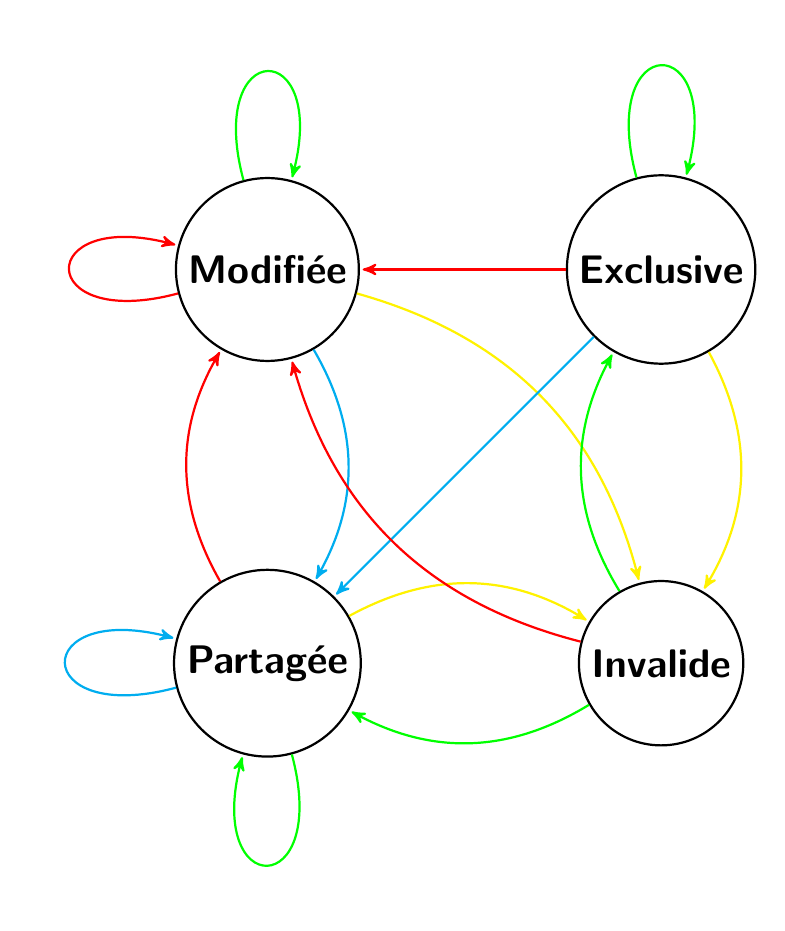
\begin{tikzpicture}[-,>=stealth',shorten >=1pt,auto,node distance=5cm,
  thick,main node/.style={circle,draw,font=\sffamily\Large\bfseries}]

	\node[main node] (1) {Modifiée};
    \node[main node] (2) [right of=1] {Exclusive};
    \node[main node] (3) [below of=1] {Partagée};
    \node[main node] (4) [right of=3] {Invalide};
    
    \path (1) edge [cyan, ->, bend left] (3);
    \path (1) edge [yellow, ->, bend left] (4);
    \path (1) edge [green, ->, loop above] (1);
    \path (1) edge [red, ->, loop left] (1);
    \path (2) edge [green, ->, loop above] (2);
    \path (2) edge [red, ->] (1);
    \path (2) edge [cyan, ->] (3);
    \path (2) edge [yellow, ->, bend left] (4);
    \path (3) edge [red, ->, bend left] (1);
    \path (3) edge [yellow, ->, bend left] (4);
    \path (3) edge [cyan, ->, loop left] (3);
    \path (3) edge [green, ->, loop below] (3);
    \path (4) edge [red, ->, bend left] (1);
    \path (4) edge [green, ->, bend left] (2);
    \path (4) edge [green, ->, bend left] (3);

\end{tikzpicture}
}
\end{center}
\begin{textblock}{5}(1, 7.8)
\textcolor{red}{Écriture locale} \\
\textcolor{green}{Lecture locale} \\
\textcolor{cyan}{Lecture distante} \\
\textcolor{yellow}{Écriture distante}
\end{textblock}
\end{frame}

\section{Modèle insensible à la cache}
\subsection{Concept}
\begin{frame}
\frametitle{Concept}
\begin{columns}
    \begin{column}{0.5\textwidth}
\begin{itemize}
\item Conscience de l'existence d'une cache
\item Inconscience des détails spécifiques
\end{itemize}
    \end{column}
    \begin{column}{0.5\textwidth}
\begin{center}
\begin{tikzpicture}[-,>=stealth',shorten >=1pt,auto,node distance=3cm,
  thick,main node/.style={circle,draw,font=\sffamily\Large\bfseries}]

    \draw[white] (0, 0) rectangle (4, 0.75);
    \draw[white] (0, 0.75) rectangle (4, 1.5);
    \draw[white] (0, 1.5) rectangle (4, 2.25);
    \draw[white] (0, 2.25) rectangle (4, 3);
    \draw[white] (0, 3) rectangle (4, 3.75);
    \draw[white] (0, 3.75) rectangle (4, 4.5);
    
    \draw[white] (-0.1, -0.03) -- (-0.3, -0.03) -- (-0.3, 4.5) -- (-0.1, 4.5) node (1) at (-0.7, 2.4) {$M$};
    
    \draw[white] (0, -0.1) -- (0, -0.3) -- (4, -0.3) -- (4, -0.1) node (1) at (2, -0.6) {$B$};
   
\end{tikzpicture}
\end{center}
    \end{column}
\end{columns}
\end{frame}

\subsection{Algorithmes}
\begin{frame}
\frametitle{Algorithmes}
\begin{itemize}
\item
\end{itemize}
\end{frame}

\begin{frame}[fragile]
\frametitle{Multiplication de matrices}
\framesubtitle{Approche traditionnelle}
\begin{lstlisting}
for (int i = 0; i < N; ++i)
  for (int j = 0; j < N; ++i)
    for (int k = 0; k < N; ++k)
      C[i][j] += A[i][k] * B[k][j];
\end{lstlisting}
\end{frame}

\begin{frame}[fragile]
\frametitle{Multiplication de matrices}
\framesubtitle{Approche optimisée}
\begin{lstlisting}
for(int i_0 = 0; i_0 < N; i_0+=b)
  for(int j_0 = 0; j_0 < N; i_0+=b)
    for (int i = i_0; i < min(i_0+b, N); ++i)
      for (int j = j_0; j < min(j_0+b, N); ++j)
        for(int k = 0; k < N; ++k)
          C[i][j] += A[i][k] * B[k][j];
\end{lstlisting}
\end{frame}

\begin{frame}[fragile]
\frametitle{Multiplication de matrices}
\framesubtitle{Approche insensible à la cache}
\begin{lstlisting}
for(int i = 0; i < N; ++i) {
  for(int j = 0; j < N; ++i) {
    for(int k = 0; k < N; ++k) {
      C[i][j] += A[i][k] * B[k][j];
    }
  }
}
\end{lstlisting}
\end{frame}

\subsection{Structures de données}
\begin{frame}
\frametitle{Structures de données}
\begin{itemize}
\item
\end{itemize}
\end{frame}

\begin{frame}
\frametitle{Arbre de van Emde Boas}
\begin{center}
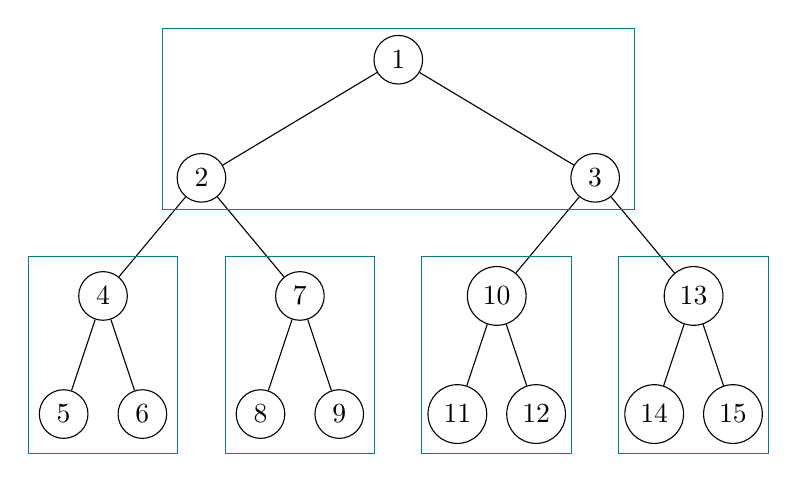
\begin{tikzpicture}[level distance=1.5cm,
level 1/.style={sibling distance=5cm},
level 2/.style={sibling distance=2.5cm},
level 3/.style={sibling distance=1cm}]
\tikzstyle{every node}=[circle,draw]

\node (Root) {1}
    child {
    node {2} 
    child { node {4}
    		child { node {5} }
    		child { node {6} } 
    }
    child { node {7}
    		child { node {8} }
    		child { node {9} }
    }
}
child {
    node {3}
    child { node {10} 
    		child { node {11} }
    		child { node {12} }
    }
    child { node {13} 
    		child { node {14} }
    		child { node {15} }
    }
};

\draw[teal] (-3, 0.4) rectangle (3, -1.9);
\draw[teal] (-4.7, -2.5) rectangle (-2.8, -5);
\draw[teal] (-2.2, -2.5) rectangle (-0.3, -5);
\draw[teal] (0.3, -2.5) rectangle (2.2, -5);
\draw[teal] (2.8, -2.5) rectangle (4.7, -5);

\end{tikzpicture}
\end{center}
\end{frame}

\section{Conclusion}
\begin{frame}
\frametitle{Conclusion}
\begin{itemize}
\item Les meilleures performances proviennent souvent d'un programme conscient de la cache.
\item<2-> Une façon d'exploiter la localité est d'utiliser des algorithmes et des structures de données insensibles à la cache.
\item<3-> Les algorithmes insensibles à la cache offrent des opportunités de parallélisation.
\end{itemize}
\end{frame}

\end{document}